% https://www.actual.world/resources/courses/spring-15/latex/
\documentclass[12pt]{article}

\usepackage{amsmath,amssymb} % essential packages for math symbols

\usepackage{tikz,pgf} % for drawing diagrams
\usetikzlibrary{arrows,positioning,decorations.pathmorphing} % for drawing arrows in diagrams
\tikzset{snake it/.style={-stealth,
    decoration={snake, 
        amplitude = .4mm,
        segment length = 2mm,
        post length=0.9mm},
    decorate}}

\begin{document}

\title{Example Diagrams with PGF/TikZ}
\date{}

\maketitle

\begin{center}
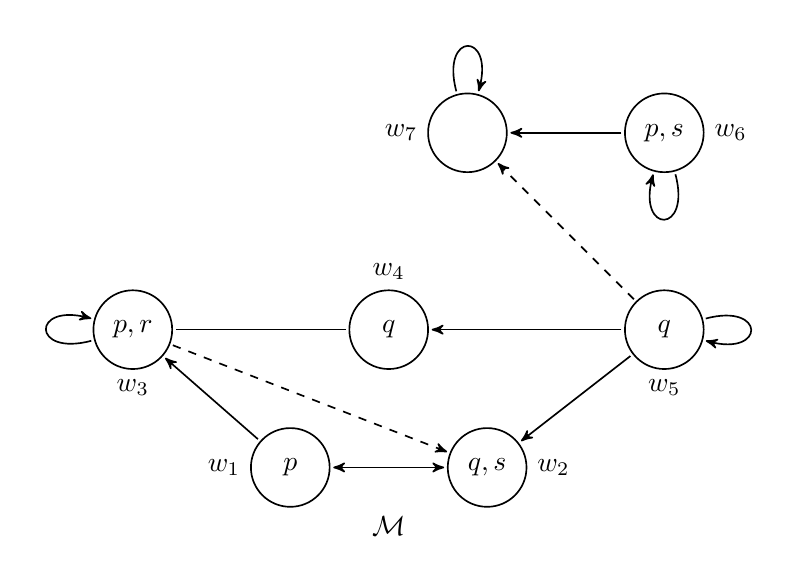
\begin{tikzpicture}[->,>=stealth',shorten >=1pt,shorten <=1pt, auto,node
distance=2.5cm,semithick]
\tikzstyle{every state}=[fill=gray!20,draw=none,text=black]
\node[circle,draw=black!100,label=left:$w_1$,minimum size=1cm] (w1) {{$p$ }};
\node[circle,draw=black!100,label=right:$w_2$,minimum size=1cm] (w2) [right of=w1] {{$q,s$}};
\node[circle,draw=black!100,label=below:$w_3$,minimum size=1cm] (w3) at (-2,1.75)  {{$p,r$}};
\node[circle,draw=black!100,label=above:$w_4$,minimum size=1cm] (w4) at (1.25,1.75)  {{$q$}};
\node[circle,draw=black!100,label=below:$w_5$,minimum size=1cm] (w5) at (4.75,1.75)  {{$q$}};
\node[circle,draw=black!100,label=right:$w_6$,minimum size=1cm] (w6) [above of=w5]{{$p,s$}};
\node[circle,draw=black!100,label=left:$w_7$,minimum size=1cm] (w7) [left of=w6]{{$$}};
\path (w1) edge[<->] node { } (w2);
\path (w1) edge[->] node { } (w3);
\path (w3) edge[loop left] node { } (w3);
\path (w5) edge[loop right] node { } (w5);
\path (w3) edge[dashed,->] node { } (w2);
\path (w4) edge[-] node { } (w3);
\path (w5) edge[->] node { } (w4);
\path (w5) edge[->] node { } (w2);
\path (w5) edge[dashed,->] node { } (w7);
\path (w6) edge[->] node { } (w7);
\path (w7) edge[loop above] node { } (w7);
\path (w6) edge[loop below] node { } (w6);

\node  at (1.25,-.75) {$\mathcal{M}$};

\end{tikzpicture}

\vspace{1cm}

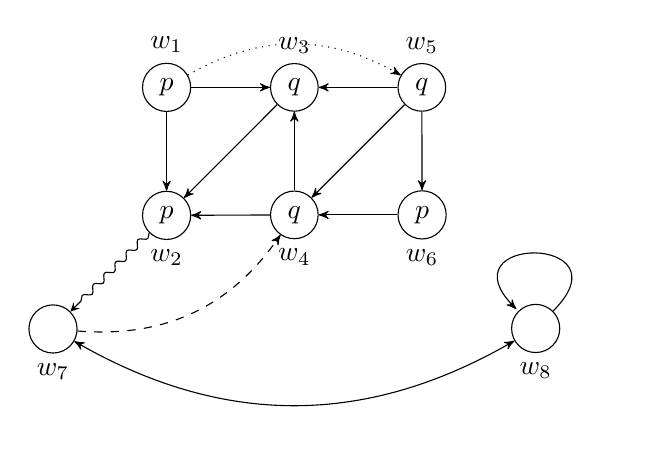
\begin{tikzpicture}[>=stealth']
  
\node (w1) [circle,draw=black,label=above:$w_1$]  {$p$}; 
\node (w2) [below=of w1,circle,draw=black,label=below:$w_2$]  {$p$}; 
\node (w3) [right=of w1,circle,draw=black,label=above:$w_3$]  {$q$};
\node (w4) [below=of w3,circle,draw=black,label=below:$w_4$]  {$q$};
\node (w5) [right=of w3,circle,draw=black,label=above:$w_5$]  {$q$};
\node (w6) [right=of w4,circle,draw=black,label=below:$w_6$]  {$p$};]
\node (w7) [below left=of w2,circle,draw=black,label=below:$w_7$] {\phantom{$p$}};
\node (w8) [below right=of w6,circle,draw=black,label=below:$w_8$] {\phantom{$p$}};

\path[->]  (w1) edge (w2);
\path[->]  (w1) edge (w3);
\path[->]  (w3) edge (w2);
\path[->]  (w4) edge (w2);
\path[->]  (w4) edge (w3);
\path[->]  (w5) edge (w3);
\path[->]  (w5) edge (w4);
\path[->]  (w5) edge (w6);
\path[->]  (w6) edge (w4);
\path[->]  (w2) edge[snake it] (w7);
\path[->]  (w8) edge[loop] (3,3);
\path[<->]  (w7) edge[bend right] (w8);
\path[->]  (w7) edge[dashed,bend right] (w4);
\path[->]  (w1) edge[dotted,bend left] (w5);
 
\end{tikzpicture}
\end{center}
	
\end{document}